% !TEX root = epifanov_solid_state_physics.tex
%!TEX TS-program = pdflatex
%!TEX encoding = UTF-8 Unicode


\chapter[The Band Theory of Solids]{The Band Theory of Solids}\label{chap:5}
% \chaptermark{The Band Theory of Solids}

The theory of free electrons was the first successful attempt to explain the electric and magnetic properties of solids (primarily of metals). It was based on the assumption that metals contain free electrons capable of moving around the metal like gas molecules in a vessel. The theory of free electrons was successful in explaining such phenomena as the electric and the heat conductivities, thermionic emission, thermoelectric and galvanomagnetic effects, etc. However, this theory proved incapable of dealing with such properties of solids as are determined by their internal structure. It could not even explain why some bodies are conductors and some insulators.

The next stage in the progress of the electron theory has been the band theory of solids, which is outlined in this chapter.

\section{Electron energy levels of a free atom}\label{sec:37}


% \begin{figure}[t]
% 	\begin{center}
% 		
\includegraphics[scale=1.1]{figures/ch_04/fig_4_1.pdf}
% 		\caption[]{}
% 		\label{fig:4_1}
% 	\end{center}
% 	\vspace{-0.7cm}
% \end{figure}

% \begin{figure}[t]
% 	\begin{minipage}[t]{0.52\linewidth}
% 		\begin{center}
% 			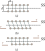
\includegraphics[scale=1]{figures/ch_02/fig_2_7.pdf}
% 			\caption[]{Diagram of rigid shear: (a) --- equilibrium position of atoms in atomic planes adjoining the slip plane; (b) --- gradual shift of one plane in relation to another caused by external stress $\tau$; (c) --- lower atomic plane as a whole displaced by one interatomic distance in relation to the upper plane.}
% 			\label{fig:2_7}
% 		\end{center}
% 	\end{minipage}
% 	\hfill{ }%\hspace{-0.1cm}
% 	\begin{minipage}[t]{0.43\linewidth}
% 		\begin{center}
% 			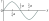
\includegraphics[scale=1]{figures/ch_02/fig_2_8.pdf}
% 			\caption[]{Variation of resistance to shear in the process of displacement of one part of the lattice in relation to another.}
% 			\label{fig:2_8}
% 		\end{center}
% 	\end{minipage}
% \vspace{-0.3cm}
% \end{figure}

% \begin{table}[!b]
% 	\renewcommand{\arraystretch}{1.2}
% 	\caption{}
% 	\vspace{-0.6cm}
% 	\label{table:4_3}
% 	\begin{center}\resizebox{0.75\linewidth}{!}{
% 			\begin{tabular}{lclc}
% 				\toprule[1pt]
% 				\textbf{Metal} & $\mathscr{K}, \parenthesis{\si{\watt\per\metre\per\kelvin}}$ & \textbf{Metal} & $\mathscr{K}, \parenthesis{\si{\watt\per\metre\per\kelvin}}$\\
%                 \midrule[0.5pt]\midrule[0.5pt]
%                 Silver & $403$ & Aluminium & $210$\\
%                 Copper & $384$ & Nickel & $60.0$\\
%                 Gold & $296$ & Constantan & $23.0$\\
% 				\bottomrule[1pt]
% 			\end{tabular}
% 	}\end{center}
% \end{table}
